	\section{MILP Models for Global Robustness}

Let $N$ the number of neurons of a DNN. Compared with local robustness which considers only variables $(x'_j)_{j \leq N}$ for the perturbed image $I'$, global robustness considers also variables $(x_j)_{j \leq N}$ for the ({\em non}-fixed) input image $I$, and thus necessitates double the number of (binary) variables (for $I$ and for $I'$). Worst-case complexity being exponential in the number of binary variables, global robustness (e.g. ITNE and VHAGaR \cite{ITNE,vhagar}) is much harder than local robustness.

\subsection{Encoding $L_\infty$- and $L_1$-perturbations for input variables}
\label{s.L1}

To encode $L_\infty$-perturbations bounded by $\varepsilon$,
the linear constraint $|x_j-x'_j| \leq \varepsilon$ is used for each {\em input} neuron $j$. 

\smallskip

We now explain how to encode $L_1$-perturbations bounded by $\varepsilon$,
using additional variables that are linear only. Let $n$ be the number of input neurons. 
We use $n$ additional linear variables $(A_i)_{i \leq n}$, with the following  constrains:
\begin{align}\label{L1constraint}\begin{cases}
	A_j \geq x_j - x'_j &\text{ for all }j \leq n\\ 
	A_j \geq x'_j - x_j &\text{ for all }j \leq n\\
	\sum_{j\leq n} A_j \leq \varepsilon	&\end{cases}
\end{align}

\begin{proof}
%We prove that (\ref{L1constraint}) are equivalent with asking $||\vec{x}||_{L_1} = \sum_{j\leq n} |x_j-x'_j| \leq c$.

The first two lines of constraints (\ref{L1constraint}) are equivalent with $A_j \geq |x_j - x'_j|$. 
So the whole constraint (\ref{L1constraint}) 
implies that $\sum_{j\leq n} |x_j - x'_j| \leq \varepsilon$.

Conversely, for every instance that satisfies $\sum_{j\leq n} |x_j - x'_j| \leq \varepsilon$, then there is also an instance which satisfies constraints (\ref{L1constraint}),  by defining $A_j = |x_j - x'_j|$ for all $j \leq n$.

This shows that (\ref{L1constraint}) is equivalent with 
$||\vec{x} - \vec{x}'||_{L_1} = \sum_{j\leq n} |x_j-x'_j| \leq \varepsilon$.
\qed
\end{proof}


\subsection{Constraints for propagation in the DNN}


There are two kinds of propagation of values for variables: 
for a neuron $j$ of layer $\ell$, the value of variable $x_j$ is defined by the constraint $x_j = \sum_{i \in \ell-1} \alpha_i \hat{x_i}$, which is a simple linear operation from the output $(\hat{x_i})_{i \in \ell-1}$ of neurons $i$ in layer $\ell-1$.

In the same way, $x'_j = \sum_{i \in \ell-1} \alpha_i \hat{x}'_i$ 
for variable $x'_j$ associated with the perturbed image $I'$, using the same $\alpha_i$ associated with the DNN weights. Similarly, 
if the {\em Diff} variables $y_j = x'_j - x_j$ are considered as defined in Section 2, with $\hat{y}_j = \hat{x}_j - \hat{x}'_j$, then we simply have 
$y_j = \sum_{i \in \ell-1} \alpha_i \hat{y}_i$.

It remains to consider the (non-linear) ReLU functions from $x_j,x'_j$ and/or $y_j$ to $\hat{x_j},\hat{x}'_j$ and/or $\hat{y}_j$, which is the complex part, with different possible solutions explored in the following with different set of variables considered. 



		%(see later how we encode $L_1$ perturbations).


	
\subsection{The classical encoding of ReLUs for global robustness}
	
    The classical encoding is used (with variants) by VHAGaR \cite{vhagar} and ITNE \cite{ITNE}. For each neuron $j$, variables $x_j,\hat{x}_j$ and $x'_j,\hat{x}'_j$ are considered. For each ReLU $j$, a binary variable $a_j$ and related constraints from the classical encoding (\ref{eq11}) \cite{MILP} are used to set $\hat{x}_j$, and an {\em independent} binary variable $a'_j$ and related constraints from the classical encoding are used to set $\hat{x}_j$. We call this encoding $\mathcal{M}^{classical}$.
	
	As explained in the section \ref{s.notation}, the standard way to make the MILP model more efficient is to linearly relax some of the binary variables into linear variables. The problem is that the LP relaxation of this classical encoding is extremely inaccurate, as variables $x_j,x'_j$ dependencies are due solely on the function definition through common ancestor variables in previous layers - as this is approximated with LP, most of the dependencies will be lost. On top of being an issue with partial MILP models, LP relaxation is also used during the Branch and Bound process internal to MILP solvers to provide bounds for each branch. So even when 
	no LP relaxation is used, the classical MILP encoding of \cite{MILP}, while asymptotically accurate, will result into looser bounds in practice. 
	
	To improve this, ITNE adds some linear constraints to the model (Eq. (3) in \cite{ITNE}, see also Section \ref{s.diff}), while VHAGaR reduces the number of binary variables depending on the perturbation used \cite{vhagar}.
	
	
	%We will compare the different methods in Table \ref{table.classical}.


	
	
	


	
	%It contains twice as many variables as for local robustness. 
	%As the worst-case complexity of solving an MILP model is exponential in the number of binary variables, it will be computationally intractable to compute $\beta^\varepsilon_{i,j}$ in this way, but for very small DNNs. 


	\subsection{The novel {\em Diff} MILP encoding for global robustness}
	\label{s.diff}

	We now present our main methodological contribution, the {\em Diff} MILP encoding. It considers variables $x'_j,\hat{x}'_j, y_j, \hat{y}_j$, where $y_j, \hat{y}_j$ are the {\em Diff variables} \cite{diff}, with 
	$y_j = x_j - x'_j$ and $\hat{y}_j= \ReLU({x}_j) - \ReLU(x'_j)$. 
	A first important observation is that the image $I$ and the deformation $I'$ having perfectly symmetrical roles, assuming that $\gamma_j$ is an {\em upper} bound of $y_j$, then $-\gamma_j$ is a {\em lower} bound for $y_j$.


	To encode the equation describing $\hat{x}'_j$, we use 
	the MILP constraints from the classical encoding (\ref{eq11}), including
	one binary variable $a'_j$, similar to ITNE.

    However, unlike ITNE, 
	%Interleaving Twin-Network Encoding (ITNE) of \cite{lipshitz,ITNE} which relies on the classical MILP encoding (\ref{eq11}) \cite{MILP} to compute $\hat{y}_j$ from the difference between 
	%$\ReLU(x'_j + y_j) = \ReLU(x_j) = \hat{x_j}$
	%and $\hat{x}'_j$, 
	the {\em Diff} MILP model encodes the equation for $\hat{y}_j$ directly, without resorting to the classical encoding from $x_j(=y_j+x'_j)$ to 
	$\ReLU(x_j)$ and using $\hat{y}_j= \ReLU(x_j) - \ReLU(x'_j)$, which is correct but does not encode explicitly that $\hat{y}_j$ is small when $y_j$ is small, since both ReLUs can be large and they are encoded independently, see also \cite{diff}. Instead, we study the function from $(x'_j,y_j)$ to $\hat{y}_j$, and encode it into the novel MILP {\em Diff} model.
    


	%	(This model has the same binary set, although the meaning of binary variable for $y_i$ is somehow different.)
	
	%	The exact constraints for $$ \begin{align*}
		%		&\hat{y}_i \geq -\hat{x}'_i \hspace*{1ex} \wedge \hspace*{1ex} \hat{y}_i \leq -\hat{x}'_i+a\beta_i  \hspace*{1ex}\wedge\hspace*{1ex} x_i'+y_i \leq a\beta_i \hspace*{1ex}\wedge\hspace*{1ex}  x_i'+y_i \geq (1-a)\alpha_i \\
		%		&\hat{y}_i \geq -\hat{x}'_i+(x_i'+y_i) \hspace*{1ex}\wedge\hspace*{1ex} \hat{y}_i \leq -\hat{x}'_i+(x_i'+y_i) +(a-1)\alpha_i \\
		%	\end{align*} 
	%	
	%	
	%	Moreover, we can add two more natural constraints: $x_i'+y_i \geq \alpha_i \hspace*{1ex}\wedge\hspace*{1ex}  x_i'+y_i \leq \beta_i.$
	
	We first display on Figure \ref{fig.2v} the function $f(x'_j,y_j)=\hat{y}_j$ for $y_j \in [- \gamma_j, \gamma_j]$. 
	When $x'_j \leq 0$ and $x_j = x'_j+y_j \leq 0$, we have $\hat{y}_j = \ReLU(x_j) - \ReLU(x'_j) = 0-0=0$. For $x'_j \geq 0$ and $x_j = x'_j+y_j \geq 0$, we have $\hat{y}_j= \ReLU(x_j)-\ReLU(x'_j)=x_j - x'_j = y_j$. 
    Between these two linear planes, we have two more linear planes presenting intermediate cases, so 4 linear planes in total.
	
	\begin{figure}[b!]
		\centering
	\hspace*{-5ex}
	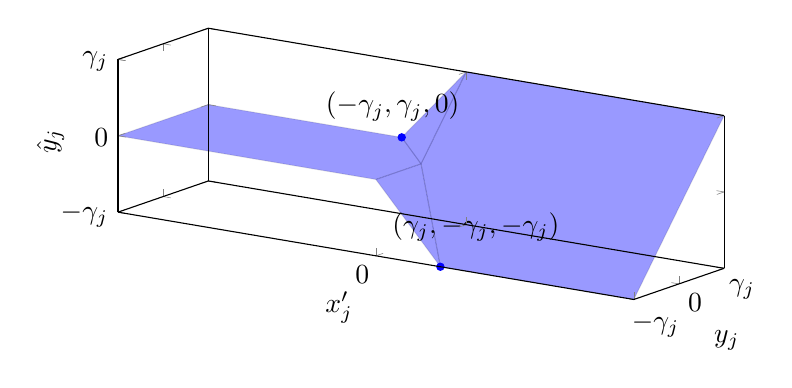
\begin{tikzpicture}[scale=0.65]
		\begin{axis}[	axis on top, xlabel = \(x'_j\),
			ylabel = {\(y_j\)}, zlabel = \(\hat{y}_j\),
			set layers=default,
			xmax = 4, xmin = -4,
			ymax = 1, ymin = -1,		
			zmax = 1, zmin = -1,
			unit vector ratio=1 1 1, scale=2.5,  ytick   = {-1,0,1},
			yticklabels = {$-\gamma_j$,$0$,$\gamma_j$}, xtick = {0},
			xticklabels = {$0$}, ztick   = {-1,0,1},
			zticklabels = {$-\gamma_j$,$0$,$\gamma_j$},
			view={35}{14},
			]
			\addplot3[ fill=blue,opacity=0.1, fill opacity=0.4] 
			coordinates {
				(0,0,0) (-1,1,0) (-4,1,0) (-4,-1,0) (0,-1,0) (0,0,0)
			};
			
			\addplot3[	fill=blue,opacity=0.1, fill opacity=0.4] 
			coordinates { (0,0,0) (0,1,1) (4, 1, 1) (4, -1, -1) (1,-1,-1) (0,0,0)
			};
			
			\addplot3[	fill=blue,opacity=0.1, fill opacity=0.4	] 
			coordinates { (0,0,0)  (-1,1,0) (0,1,1) (0,0,0)
			};
			
			\addplot3[	fill=blue,opacity=0.1, fill opacity=0.4	] 
			coordinates { (0,0,0)  (0,-1,0) (1,-1,-1) (0,0,0)
			};
			
			\addplot3[only marks, mark=*, mark size=2pt, blue] coordinates {(1,-1,-1)};
			\node[label={$(\gamma_j,-\gamma_j, -\gamma_j)$}] at (axis cs: 1.2, -0.5 ,-1) {};
			
			\addplot3[only marks, mark=*, mark size=2pt, blue] coordinates {(-1,1,0)};
			\node[label={$(-\gamma_j,\gamma_j, 0)$}] at (axis cs: -1, 0.8 ,0) {};			
		\end{axis}
	\end{tikzpicture}
	\caption{The function computing $\hat{y}_j=\ReLU(x_j=y_j+x'_j)-\ReLU(x'_j)$ 
	depending on $y_j$ and on $x'_j$.}
	\label{fig.2v}
\end{figure}
	

Recall first that $a'_j$ is the binary variables used in the 
 classical MILP encoding for $\hat{x}'_j=\ReLU(x'_j)$.
We set $a'=a'_j$ (whose value is already settled, see Proposition \ref{Prop1}),
and use it in the MILP encoding of $\hat{y}_j = \ReLU(x_j)-\ReLU(x'_j)$:

\newpage

\begin{proposition}
    \label{Prop2}
Assuming $y_j \in [-\gamma_j, \gamma_j]$ and $x'_j \in [\alpha_j,\beta_j]$, we have that $\hat{y}_j = \ReLU(x_j=y_j + x'_j) - \ReLU(x'_j)$ is the solution of the MILP program:
	\begin{align*}
		& \begin{aligned}
			y_j + x'_j &\leq a\beta_j        &
			y_j &+ x'_j \geq (1-a)\alpha_j \\
			x'_j       &\leq a'\beta_j       & 
			x'_j       &\geq (1-a')\alpha_j \\
			\hat{y}_j  &\leq a\gamma_j       &
			\hat{y}_j  &\geq -a'\gamma_j \\
			\hat{y}_j  &\leq y_j + x'_j + (1-a)(-\alpha_j) &
			\hat{y}_j  &\geq y_j + x'_j + a'(-\beta_j) \\
			\hat{y}_j  &\leq -x'_j + a\beta_j &
			\hat{y}_j  &\geq -x'_j + (1-a')\alpha_j \\
			\hat{y}_j  &\leq y_j + (1-a)\gamma_j  &
			\hat{y}_j  &\geq y_j - (1-a')\gamma_j
		\end{aligned}
	\end{align*} 
    where $a,a' \in \{0,1\}$ are binary variables, 
    and $a'$ is shared with the classical MILP
    encoding for $\hat{x}'_j=\ReLU(x'_j)$.
\end{proposition}

So to encode both $\hat{y}_j$ and $\hat{x}'_j$, the {\em Diff} encoding needs 2 binary variables, similar to the classical encoding for $\hat{x}_j$ and $\hat{x}'_j$. 

\begin{proof}
First, we know the constraints for $\hat{x}_j'=\ReLU(x_j')$ are exact, by Prop \ref{Prop1}. We now do a case analysis depending on the value of both binary variables. 
%We have 2 binary variables and 4 cases in total.
 We check that in all 4 cases $\hat{y}_j = \ReLU(y_j+x'_j)-\ReLU(x'_j)$.

\textbf{$\mathbf{a = 0, a' = 0}$:}  In this case $y_j+x'_j\leq 0$ and $x'_j \leq 0 $ (lines 1\&2). We thus have to show that 
$\hat{y}_j = 0$. This is true thanks to inequalities in line 3.

\textbf{$\mathbf{a = 1, a' = 0}$:}  In this case $y_j+x'_j\geq 0$ and $x'_j \leq 0$ (lines 1\&2). We thus have to show that 
$\hat{y}_j = y_j+x'_j$. This is true thanks to inequalities in line 4.

\textbf{$\mathbf{a = 0, a' = 1}$:}  In this case $y_j+x'_j\leq 0$ and
$x'_j \geq 0 $ (lines 1\&2). We thus have to show that 
$\hat{y}_j = -x'_j$. This is true thanks to inequalities in line 5.

\textbf{$\mathbf{a = 1, a' = 1}$:} 
In this case, $y_j+x'_j\geq 0$ and $x'_j \geq 0 $ (lines 1\&2). We thus have to show that $\hat{y}_j = y_j$. This is true thanks to inequalities in line 6.

Notice that in each case, equations not mentioned are moot.
	\qed
\end{proof}


%The proof of Prop. \ref{Prop2} can be found in the supplementary materials.

Intuitively, the {\em diff values} will be small as they will be carrying the difference between the image $I$ and its slight perturbation $I'$.
The LP relaxation of ${\cal M}^{classical}$ will miss this totally, while the LP relaxation of the Diff model contains such important bounds, including (see 
section \ref{s.1b} and Fig.~\ref{fig.1v}):
\begin{align}
	\label{eq.lpr}
\frac{y_j-\gamma_j}{2} \leq \hat{y}_j \leq \frac{y_j+\gamma_j}{2}
\end{align}
%which is not the case of ${\cal M}^{classical}$. 
This is a simplification (due to the noticed symmetry) of the additional linear constraint (3) of \cite{ITNE} used explicitly in ITNE.
	

	\iffalse
\paragraph{A proof of Prop.~\ref{Prop2}}

We do a case analysis depending on the value of both binary variables. 
First, we know the constraints for $\hat{x_i}'=\ReLU(x_i')$ are exact (see 
Prop.~\ref{Prop1}). 

We have 2 binary variables and 4 cases in total. We only need to check that, in all 4 cases, $$\hat{y}_i = \ReLU(x'_i+y_i)-\ReLU(x'_i).$$

Case 1: if $a = 1$ and $a' = 1$, then $x'_i \geq 0 $ and $y_i+x'_i\geq 0$, then we need to show $\hat{y}_i = y_i$ based on  $\hat{x'_i} = x'_i$. This is true by the two inequalities in line 4.

Case 2: if $a = 1$ and $a' = 0$, then $x'_i \leq 0 $ and $y_i+x'_i\geq 0$, then we need to show $\hat{y}_i = y_i+x'_i$ based on  $\hat{x'_i} = 0$. This is true by the two inequalities in line 6.

Case 3: if $a = 0$ and $a' = 0$, then $x'_i \leq 0 $ and $y_i+x'_i\leq 0$, then we need to show $\hat{y}_i = 0$ based on  $\hat{x'_i} = 0$. This is true by the two inequalities in line 3.


Case 4: if $a = 0$ and $a' = 1$, then $x'_i \geq 0 $ and $y_i+x'_i\leq 0$, then we need to show $\hat{y}_i = -x'_i$ based on  $\hat{x'_i} = x'_i$. This is true by the two inequalities in line 5.

\fi

%\begin{proof}

%\end{proof}
	
	%	\begin{align*}
		%		& y_i+x'_i \leq a\beta_i \quad\wedge \quad y_i+x'_i\geq (1-a)\alpha_i\\	
		%		& x_i' \leq a'\beta_i \quad\wedge \quad x_i'\geq (1-a')\alpha_i\\
		%		&\hat{y}_i \leq a\gamma_i \quad\wedge \quad	\hat{y}_i \geq -a'\gamma_i \\
		%		&	\hat{y}_i \leq y_i+(1-a)\gamma_i \quad\wedge \quad	\hat{y}_i \geq y_i - (1-a')\gamma_i \\
		%		&	\hat{y}_i \leq -x'_i+a\beta_i \quad\wedge \quad	\hat{y}_i \geq -x'_i+(1-a')\alpha_i \\
		%		&	\hat{y}_i \leq y_i+x'_i+(1-a)(-\alpha_i)\quad\wedge \quad	\hat{y}_i \geq y_i+x'_i+a'(-\beta_i) \\
		%	\end{align*} 
	
	

	%	The relaxation of this model is similar: let $a$s and $a'$s be continuous variables instead of binary/integer variables. Unlike the first model in this section, relaxing a few nodes does not lose too much accuracy.


	\iffalse

\subsection{Comparison between classical and Diff MILP models}


Intuitively, the {\em diff values} will be small as they will be carrying the difference between both the image $I$ and its perturbation $I'$.
    

	As explained in the previous section, the standard way to make the model more efficient is to rely on linearly relaxing some of the binary variables into linear variables.
    The problem is that the LP relaxation of this classical encoding is extremely inaccurate, as variables $x_j,x'_j$ dependencies are due solely on the function definition through common ancestor variables in previous layers - as this is approximated with LP, most of the dependencies will be lost. On top of being an issue with partial MILP models, LP relaxation is also used during the Branch and Bound process internal to MILP solvers to provide bounds for each branch. So even when all variables are binary, the classical MILP encoding 
	of \cite{MILP}, while fully accurate, will likely result into looser bounds as well. Notice that this was already witnessed in \cite{ITNE}, and some additional constraints were added to make the classical model more accurate:
	the {\em diff variables} were used as specific constraints added to the classical encoding (Eq. (3) in \cite{ITNE}). 
	%We will compare the different methods in Table \ref{table.classical}.

	\fi
	

 


	
    
    
    


    \subsection{A decoupled {\em 2b+1} model}

	We propose a variant of the {\em Diff} encoding: 
	the binary variables $a'$ appearing in 
    Prop. \ref{Prop2} can be decoupled from the binary variable $a'_j$
	appearing in the classical encoding of $\hat{x}'_j = \ReLU(x'_j)$. 
	This would mean having 3 binary variables, which would be too costly. 
	The variables $a'_j$ used for $x'_j$ is thus linearly relaxed, while
	both variables $a,a'$ used in the encoding of $\hat{y}_j$ are kept binary. We call this the {\em 2b+1} model, which uses 2 binary variables per neuron, 
	as the classical and {\em Diff} encodings.
	The decoupling between $a'$ and $a_j$ removes complicated constraints in the MILP encoding, which helps the solver. This however also means that  the {\em 2b+1} model is not as accurate as the {\em Diff} model asymptotically.


	\subsection{The efficient {\em 1b} model}
	\label{s.1b}

		\begin{figure}[t!]
		\centering
	\hspace*{10ex}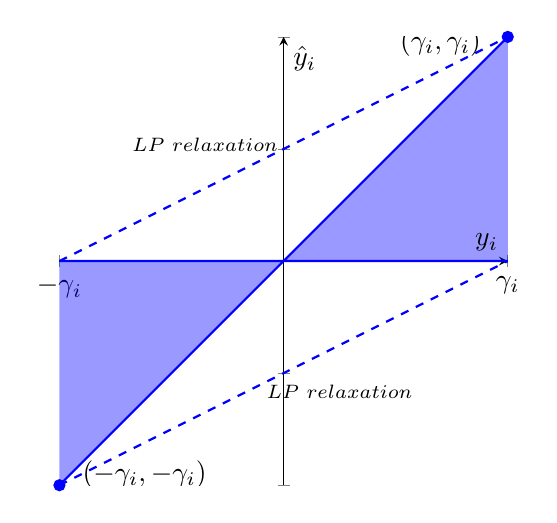
\begin{tikzpicture}
		\begin{axis}[
			xlabel={$y_i$},
			ylabel={$\hat{y}_i$},
			xmin=-2, xmax=2,
			ymin=-2, ymax=2,
			axis lines=center,
			samples=100, 
			unit vector ratio=1 1 1, scale=1, xtick   = {-2,2},
			xticklabels = {$-\gamma_i$,$\gamma_i$},
			yticklabels = {},
			]
			\addplot[blue, thick, fill=blue, fill opacity=0.4] {x} \closedcycle; 
			\addplot[blue, thick] {0}; 
			
			\addplot[only marks, mark=*, mark size=2pt, blue] coordinates {(-2,-2)};
			\node[label={above:$(-\gamma_i,-\gamma_i)$}] at (axis cs: -1.24, -2.2) {};
			
			\addplot[only marks, mark=*, mark size=2pt, blue] coordinates {(2,2)};
			\node[label={above:$(\gamma_i,\gamma_i)$}] at (axis cs: 1.4, 1.65) {};
		\addplot[dashed, thick, blue] coordinates {(-2,-2) (2,0)};
			\addplot[dashed, thick, blue] coordinates {(-2,0) (2,2)};
			\node[label={above:\scriptsize $LP\ relaxation$}] at (axis cs: -0.7, 0.8) {};
			\node[label={above:\scriptsize $LP\ relaxation$}] at (axis cs: 0.5, -1.4) {};
		\end{axis}
	\end{tikzpicture}
\caption{Possible values of $\hat{y}_i$ depending on $y_i$ for the {\em 1b} model.}
	\label{fig.1v}
\end{figure}



	To simplify further and limit the number of (binary) variables, 
    we introduce an efficient {\em 1b} model which only uses the diff variables $y_i,\hat{y}_i$. Again, we study the range of values $\hat{y}_i$ can take according to the value of $y_i$, as depicted in Fig.~\ref{fig.1v}. This is a projection of Fig.~\ref{fig.2v} onto $y_i,\hat{y}_i$.
    

    \begin{proposition}
    \label{prop3}
    Given $y_i \in [-\gamma_i,\gamma_i]$, 
    $\hat{y}_i$ is a solution of the MILP program :\begin{align*}
		\hat{y}_i &\leq a \gamma_i               &\quad \hat{y}_i &\geq y_i - a \gamma_i \\
		\hat{y}_i &\geq (a-1) \gamma_i           &\quad \hat{y}_i &\leq y_i + (1-a) \gamma_i
	\end{align*} where $a \in \{0,1\}$ is a binary variable.
	\end{proposition}

    We can easily check that the LP relaxation of this MILP program,
	depicted in broken lines on Fig.~\ref{fig.1v}, is exactly (\ref{eq.lpr}).
    
	As the {\em 1b} model is a projection of the {\em Diff} model and also of the {\em 2b+1} models, 	the LP relaxations of the {\em Diff} and the {\em 2b+1} models contain (\ref{eq.lpr}). 
	%Notice that (\ref{eq.lpr}) corresponds to Eq. (3) in \cite{ITNE}, 
	%which is added explicitly to the classical model in their ITNE model.
	
    
	
	

	\iffalse
	Based on above constraints, we can sketch this simplified model:
	\begin{enumerate}
		\item For each input node, each output node, and each pre-activation and post-activation node in the hidden layers,  set one variable $y_i$. 
		\item Set constraints for input nodes.
		\item Set linear constraints . In this case, since the meaning of $y_i$ is $x_i-x'_i$, this constraints will not use the bias.
		\item Between pre- and post- activation nodes, set the MILP constraint described above.
	\end{enumerate}
	
	The key point is that, although this model sets 3 variables (and their binary variables) for each node in the network, only $y_i$  contributes to the final results, and we can ignore $x_i,x_i'$ (and their binary variables) during the optimization.
	
	As a result, we can relax the binary variables used to $\hat{x}_i = \ReLU(x_i)$ and $\hat{x}'_i = \ReLU(x'_i)$.
	\fi


\newpage	
	
\section{Real-time verification}

%As explained in the introduction, 
The objective we want to compute upper and lower bounds on is 
$\beta^{\varepsilon}_{C,D} = \max_{|I-I'| \leq \varepsilon}((x_C - x'_C)- 
(x_D - x'_D)) = \max_{|I-I'| \leq \varepsilon}(y_C - y_D)$, for $x_{C,D},x'_{C,D}, y_{C,D}$ the value of the output neuron associated with class $C,D$ from input image $I$, perturbed image $I'$ or the differential between $I,I'$ respectively.

Upper bounds  $\bar{\beta}^{\varepsilon}_{C,D} \geq \beta^{\varepsilon}_{C,D}$ will allow us to verify in real-time whether a new incoming image can be certified to be robust for the perturbation. Lower bounds
$\underline{\beta}^{\varepsilon}_{C,D} \leq \beta^{\varepsilon}_{C,D}$
will allow us to evaluate how large is the gap= 
$\frac{(\bar{\beta}^{\varepsilon}_{C,D} - \underline{\beta}^{\varepsilon}_{C,D})} {\underline{\beta}^{\varepsilon}_{C,D}}$. MILP solvers, e.g. Gurobi, provide both an upper bound ("bound") $\bar{\beta}^{\varepsilon}_{C,D}$
as well as a lower bound ("solution") $\underline{\beta}^{\varepsilon}_{C,D}$.


Related bounds were proposed in \cite{vhagar}, for an evaluation purpose only (how narrow is the gap) rather than to verify robustness in real-time. 
Namely, VHAGaR \cite{vhagar} defines $\alpha^{\varepsilon}_{C,D}$, computing the perturbation necessary to switch an image classified as class $C$ into an image classified as class $D$:
\begin{align*}
	\alpha^{\varepsilon}_{C,D} &= \max_{|I-I'| \leq \varepsilon} (x_C-\max_{E\neq C}x_E) &\text{s.t. }  x'_D \geq \max_{E\neq D}x'_E \wedge x_C \geq \max_{E\neq C}x_E 
\end{align*}

Notice that  
$\alpha^{\varepsilon}_{C,D}$ is not symmetrical, while 
$\beta^{\varepsilon}_{C,D}$ is.


    
Assume we have computed (offline) $\bar{\beta}^{\varepsilon}_{C,D}$ for each $C,D$. Now in real-time:
\begin{enumerate}  
  \item[0] Run inference on the DNN to obtain the values $x_D$ of output neuron for each class D. Let $C$ be the class with maximal $x_{C}$. This is the predicted class from the DNN. This is the basic operation commonly done for DNN classification, without any change.
  \item[1] Compute for each class $D \neq C$
  a bit $b_D=1$ iff $x_D +\bar{\beta}^{\varepsilon}_{C,D} > x_C$.
  \item[2] Return "certified robust" iff $\bigvee_{D \neq C}(b_D)=0$.
\end{enumerate}

\begin{proposition}
  If "certified robust" is returned over input $I$, 
  then for all perturbed input $I'$ with  $|I - I'| \leq \varepsilon$,
  the DNN has the same decision on $I$ and on $I'$, i.e. the DNN is robust around $I$ for perturbation $\varepsilon$.
\end{proposition}

\begin{proof}
  Let $C$ be the decision of the DNN on $I$.
Assume by contradiction that $D \neq C$ is the decision on $I'$. 
  We know that 
  $x_D +\bar{\beta}^{\varepsilon}_{C,D} < x_C$
  because "certified robust" is returned over input $I$.
  That  is, $x_D - x_C +\bar{\beta}^{\varepsilon}_{C,D} < 0$

  By definition of $\bar{\beta}^{\varepsilon}_{C,D}$,
  we have $x'_D - x'_C + x_C - x_D \leq \bar{\beta}^{\varepsilon}_{C,D}$.
  ($I$ and $I'$ have symmetrical roles), 
  that is 
  $x'_D - x'_C \leq x_D - x_C + \bar{\beta}^{\varepsilon}_{C,D} < 0$.
  That is $x'_D < x'_C$, a contradiction with $D$ is the decision on $I'$.
  \qed
\end{proof}

The overhead (1,2 above) after 0 amounts to $2k-1$ operations, 
where $k=\#$Class. 
More precisely,
$(k-1)$ ADD(+), 
$(k-1)$ COMP(<) and $1$ OR($\bigvee$) of ($k-1$) bits.
That is, 19 operations in total for $k=10$ classes. This can be realized extremely fast, even on limited hardware.